% !TEX root =  ../main.tex

\section{Empirical Confirmation for Repeated Nesting}
\label{sec:exp-repeat-app}

In this section we consider a simple model with multiple levels of nesting.  The model is extended from
the one shown at the start of Section 6 in the main paper.  Specifically we consider the following model
\begin{align}
	\begin{split}
\label{eq:repeat-nest}
y^{(0)} &\sim \mathrm{Uniform}(-1,1), \\
y^{(1)} &\sim \mathcal{N}(0,1), \\
y^{(2)} &\sim \mathcal{N}(0,1), \\
f_0 \left(y^{(0)}, \gamma_1\left(y^{(0)}\right)\right)&= \log \gamma_1\left(y^{(0)}\right)\\
f_1 \left(y^{(0:1)}, \gamma_2\left(y^{(0:1)}\right)\right)&= 
\exp\left(-\left(y^{(0)}-y^{(1)}-\log \gamma_2\left(y^{(0:1)}\right)\right)\right)\\
f_2 \left(y^{(0:2)}\right)&=\exp\left(-\left(y^{(0)}-y^{(1)}-y^{(2)}\right)\right),\\
f_1 \left(y^{(0:1)}, \gamma_2\left(y^{(0:1)}\right)\right)&= 
	\frac{1}{\sqrt{2\pi}}\exp\left(-\frac{\left(y^{(0)}-y^{(1)}-\log \gamma_2\left(y^{(0:1)}\right)\right)^2}{2} \right)\\
f_2 \left(y^{(0:2)}\right)&=\frac{1}{\sqrt{2\pi}}\exp\left(-\frac{\left(y^{(0)}-y^{(1)}-y^{(2)}\right)^2}{2}\right),\\
\phi_1(y,z_1,\gamma_2) &= \sqrt{2/\pi}\exp\left(-2(y-z_1)^2\right), \\
\phi_2(y,z_1,z_2) &= \sqrt{2/\pi}\exp\left(-2(y-z_1-z_2)^2\right), \\
I &= \E_{p(y)}\left[\log\left(\E_{p(z_1)}\left[\phi_1\left(y,\log\left(\E_{
	 p(z_2)}\left[\phi_2(y,z_1,z_2)\right]\right)\right)\right]\right)\right].
\end{split}
\end{align}
Unlike the model in the main paper, this no longer has an analytical solution, but we generate a
ground truth estimate using a large run where $N_0 = 25000$, $N_1=5000$, and $N_2=1000$ giving 
a total of $1.25 \times 10^{11}$ samples.  The converge plot shown in Figure~\ref{fig:multi-nest} shows that the
theoretically expected convergence rates are observed.


\begin{figure}[t]
	\centering
	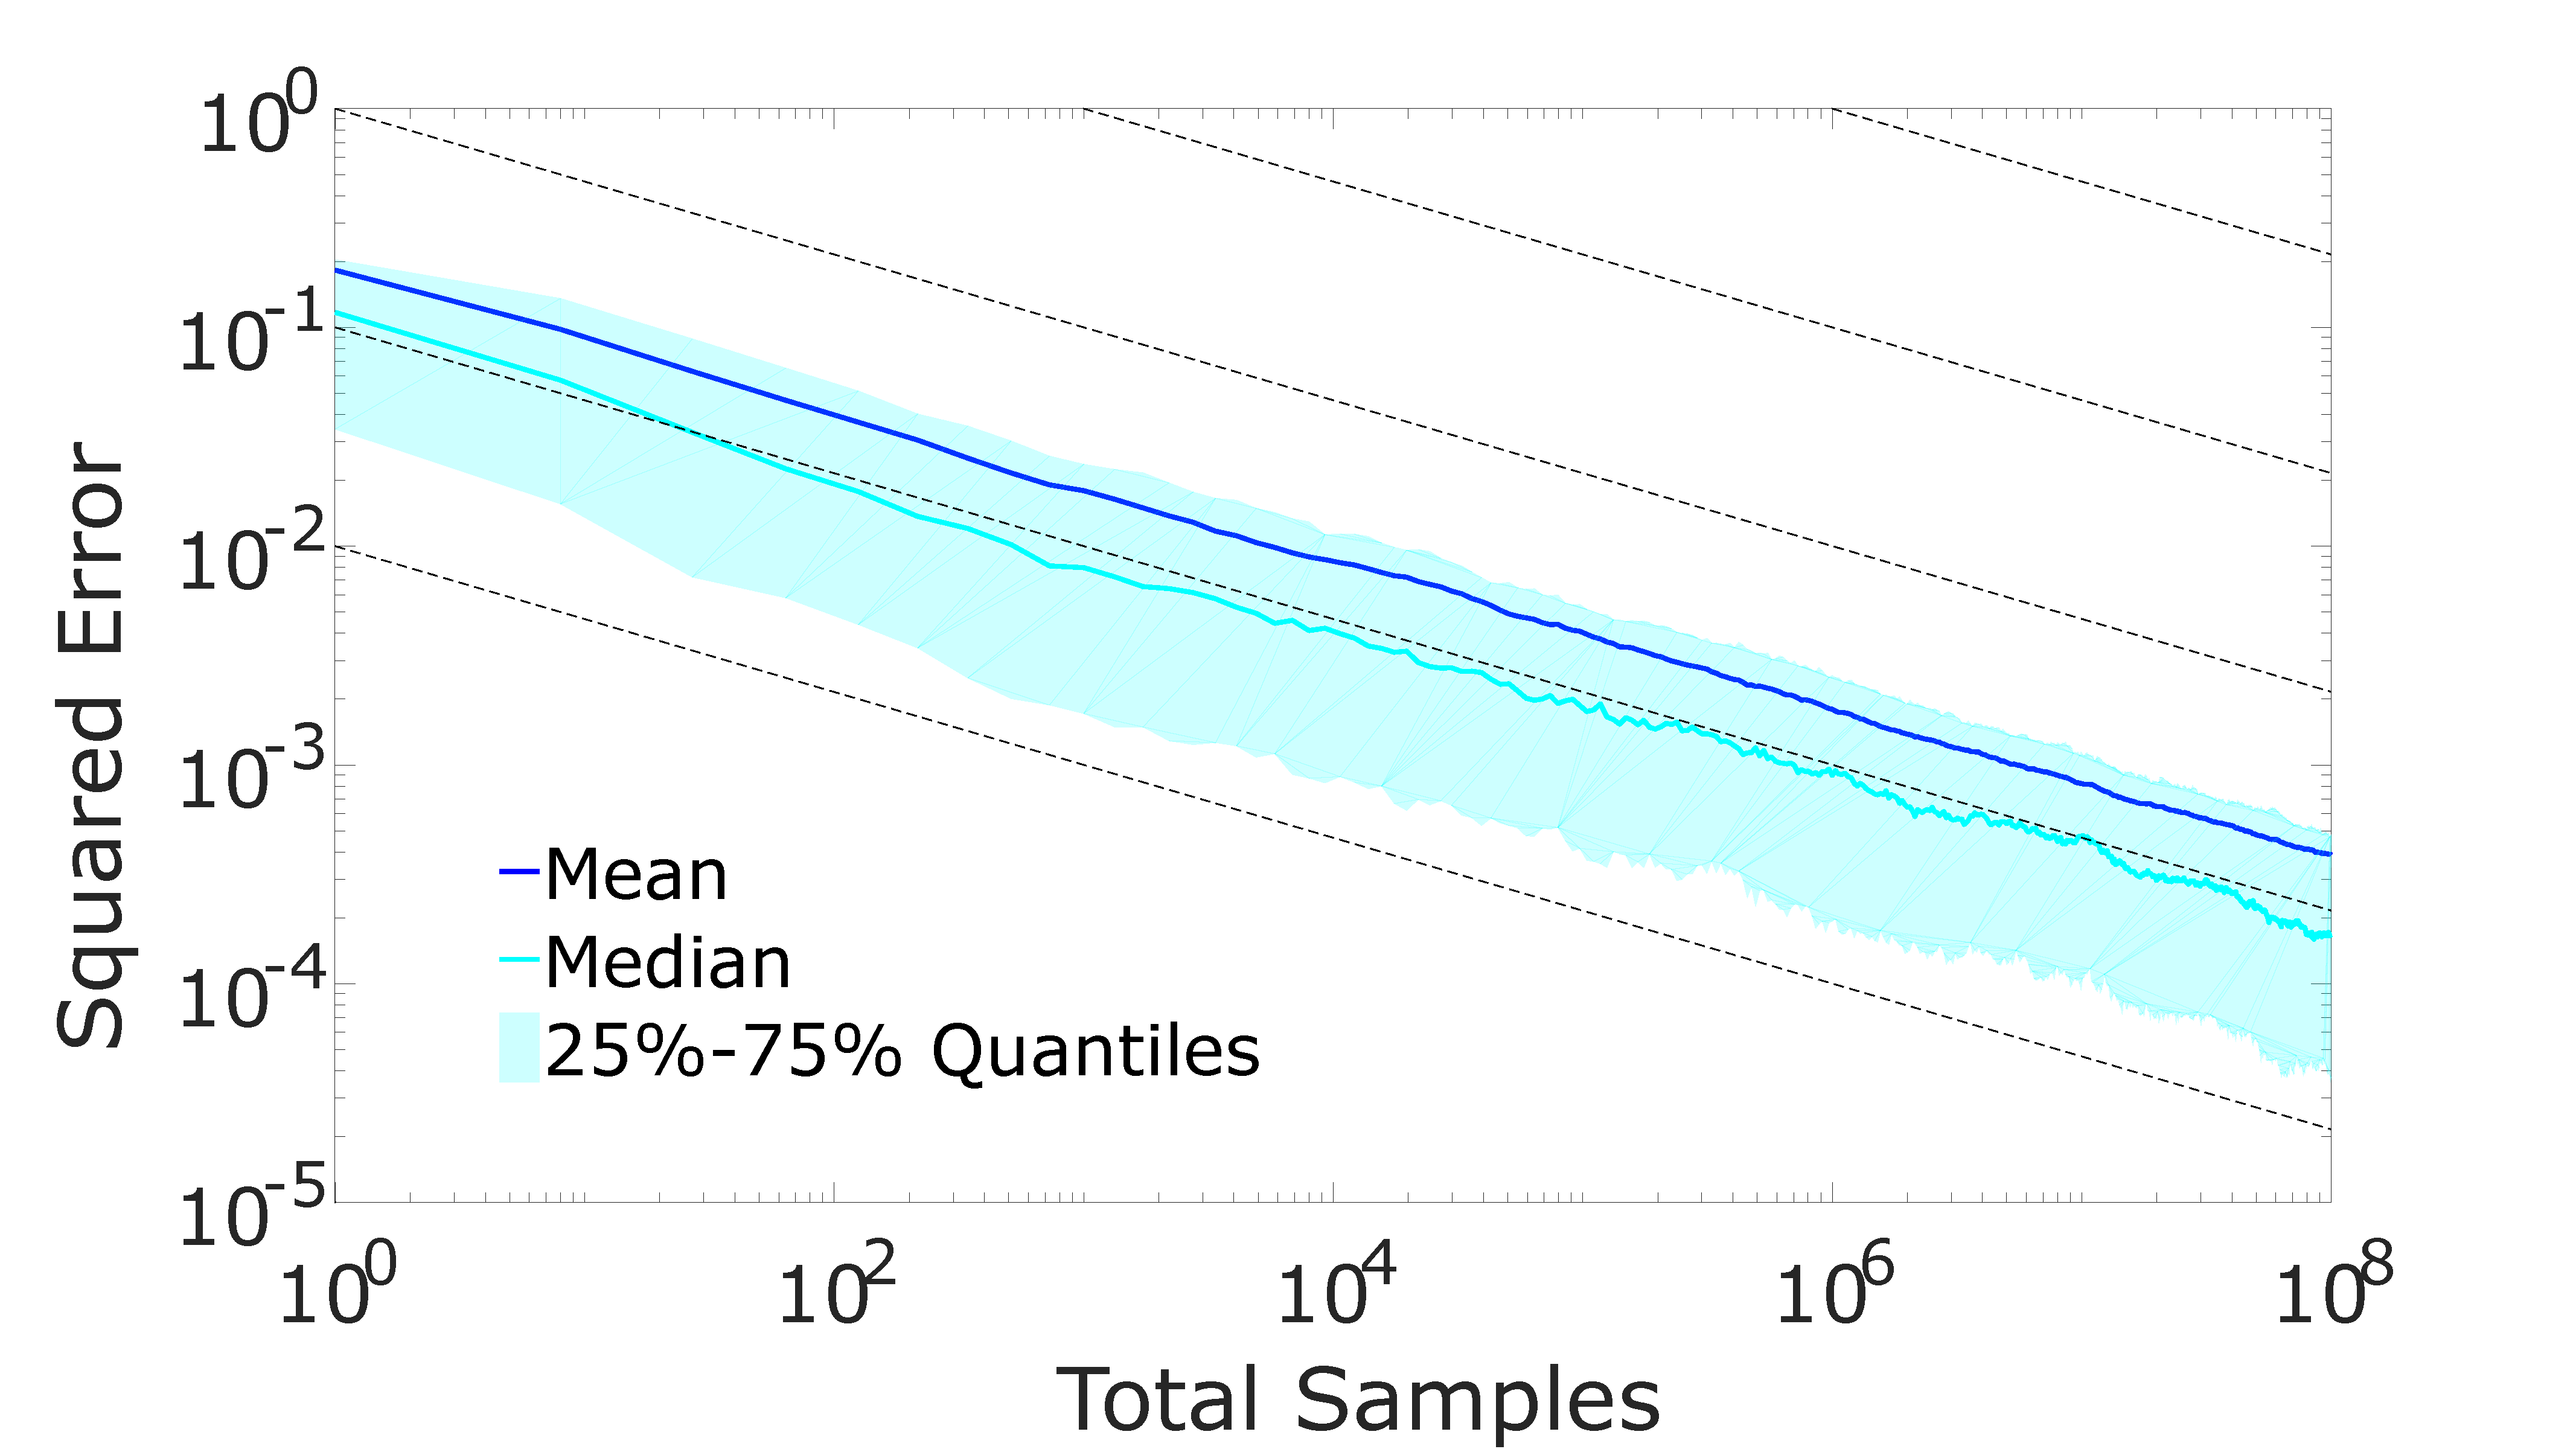
\includegraphics[width=0.6\textwidth,trim={1.5cm 0 3.5cm 0},clip]{multi_nest}
	\caption{Empirical convergence of NMC for~\eqref{eq:repeat-nest}.  We set $N_0=N_1 = N_2$ and
		observe the convergence with increasing number of total samples $T=N_0 N_1 N_2$.  We
		see the that the convergence rate suggested by our bounds of $O(T^{1/3})$ is observed as
		expected.  Results shown are from $1000$ independent runs.
		\label{fig:multi-nest}}
\end{figure}	
